\DontFrameThisInToc
\Annex{Annexe sur les assistants conversationnels (\textit{chatbots})}
\label{annex:B-ANNEXE-CHATBOTS}
	
	% INTRODUCTION DE L'ANNEXE.
	
	% Engoument pour les chatbots en 2019.
	Au début de ce doctorat (\texttt{octobre 2019}), nous pouvions noter que :
	\begin{itemize}
		\item selon \cite{costello-lodolce:2019:gartner-top-technologies}, \textguillemets{\textit{seuls $4$\% des clients de \texttt{Gartner}} [déclaraient] \textit{utiliser des \textit{chatbots} sur leur lieu de travail, mais $40$\%} [avaient] \textit{l'intention de les mettre en oeuvre à court terme}} ;
		\item et selon \cite{goasduff:2019:chatbots-will-appeal}, \textguillemets{\textit{d'ici 2022, 70\% des employés} [interagiraient] \textit{quotidiennement avec les plateformes conversationnelles}}.
	\end{itemize}
	
	% Engoument pour les chatbots en 2023.
	Aujourd'hui (\texttt{octobre 2023}), le mot \textguillemets{\textit{chatbot}} est présent sur toutes les lèvres, surtout depuis la révolution des \texttt{IA} génératives lancée par \texttt{ChatGPT} (\cite{openai:2023:chatgpt}) :
	\begin{itemize}
		\item selon \cite{costello-lodolce:2022:gartner-predicts-chatbots}, une entreprise sur deux aurait actuellement recours à une forme de \textit{chatbot} pour gérer sa relation client, et \textguillemets{\textit{d'ici 2027, les \textit{chatbots} deviendront le principal canal de service client pour environ un quart des organisations}}.
	\end{itemize}

	% Annonce du plan.
	Dans cette annexe, nous allons :
	\begin{itemize}
		\item présenter rapidement les assistants conversationnels et leurs principales utilisations (voir \textsc{Section~\ref{annex:B.1-ANNEXE-CHATBOTS-PRESENTATION}}) ;
		\item décrire les approches principales permettent de concevoir un assistant conversationnel, avec leurs avantages et leurs inconvénients (voir \textsc{Section~\ref{annex:B.2-ANNEXE-CHATBOTS-APPROCHES}}) ;
		\item discuter du dilemme des choix de conception (voir \textsc{Section~\ref{annex:B.3-ANNEXE-CHATBOTS-DILEMME}}).
	\end{itemize}
	
	% TABLE DES MATIÈRES DE L'ANNEXE.
	\minitoc
	
	
	%%%%%--------------------------------------------------------------------
	%%%%% Annexe B.1: Présentation rapide des assistants conversationnels
	%%%%%--------------------------------------------------------------------
	\newpage
	\section{Présentation rapide des assistants conversationnels}
	\label{annex:B.1-ANNEXE-CHATBOTS-PRESENTATION}
	
		%%% Fonctionnalités.
		Les \textit{chatbots} sont des robots conversationnels permettant à un utilisateur d'obtenir des informations ou d'automatiser des actions à l'aide d'instructions en langage naturel.
		\begin{itemize}
			\item[\faThumbsUp] L'utilisation de tels assistants comporte \textbf{plusieurs avantages} :
			ces derniers permettent de réduire les coûts en automatisant certaines tâches simples et répétitives (\textit{permettant aux ainsi aux humaines de se concentrer sur d'autres tâches à risques ou à forte valeur ajoutée}),
			ils sont réactifs et toujours accessibles (\textit{au milieu de la nuit, les jours fériés, et même le vendredi après 16h}),
			et ils ont un comportement stable quelle que soit la situation (\textit{pas de sauts d'humeur, de coups de fatigue ou d'erreurs d'inattention}).
			\item[\faThumbsDown] Néanmoins, ces assistants rencontrent aussi \textbf{plusieurs inconvénients} :
			leur compréhension limitée du langage peut introduire des erreurs (\textit{notamment lorsque le sujet est complexe, quand il y a trop ou trop peu de contexte}),
			ils manquent parfois de flexibilité ou d'empathie (\textit{nécessitant alors d'escalader la requête vers un opérateur humain}),
			et les tâches de conception ou de mises sous contrôle nécessitent des coûts importants (\textit{collecte et annotation de données, création de parcours de dialogue, vérification du comportement et des dérives, ...}).
		\end{itemize}
		
		
		%%% Applications.
		Ainsi, ces assistants sont utilisés dans de nombreux domaines :
		\begin{itemize}
			\item la \textbf{relation client à distance} (\textit{proposer une assistance 24/7, répondre aux questions fréquentes, automatiser la prise de rendez-vous, envoyer des formulaires de satisfaction, ...}) ;
			\item le \textbf{commerce en ligne} (\textit{remplir des formulaires de réservation ou de rétractation, suivre une commande, assurer le service après-vente, ...}) ;
			\item la \textbf{domotique} (\textit{gérer d'appareils connectés, écouter de la musique, interagir avec le \texttt{GPS}, être notifié en cas d'alerte intrusion, ...}) ;
			\item l'\textbf{accès à l'information} (\textit{consulter une base documentaire, favoriser l'éducation, vulgariser ou résumer des concepts, ...}) ; 
			\item le \textbf{divertissement} (\textit{raconter une histoire ou une blague, organiser un jeu narratif, organiser une sortie, simplement discuter lors d'une insomnie, ...}).
		\end{itemize}
		
		%%% Exemples.
		\begin{leftBarExamples}
			Parmi les exemples connus, nous avons :
			\begin{itemize}
				\item \texttt{Alexa} (\cite{alexa-internet:2018:keyword-research-competitor}) et \texttt{Google Assistant} (\cite{google:2016:google-assistant-your}), permettant de gérer des appareils connectés ;
				\item L'\texttt{Assistant Virtuel SNCF}, gérant l'achat de billets pour la SNCF (\cite{sncf:2018:agent-virtuel-sncf}) ;
				\item \texttt{Louis}, gérant le suivi des bagages d'Air France (\cite{air-france:2017:louis}) ;
				\item \texttt{AI Dungeon}, racontant des histoires interactives et des jeux de rôles (\cite{latitude-inc.-oasis-tech-inc.:2019:ai-dungeon}) ;
				\item \texttt{ChatGPT} (\cite{openai:2023:chatgpt}) ou \texttt{BARD} (\cite{google:2023:bard-chat-based}), permettant de discuter de presque n'importe quel sujet...
				\item ...
			\end{itemize}
		\end{leftBarExamples}
	
	
	%%%%%--------------------------------------------------------------------
	%%%%% Annexe B.2: Approches principales pour concevoir un \textit{chatbot}
	%%%%%--------------------------------------------------------------------
	\section{Approches de conception : \textit{task-oriented} vs \textit{chat-oriented}}
	\label{annex:B.2-ANNEXE-CHATBOTS-APPROCHES}
	
		%%% Introduction.
		Pour concevoir un assistant conversationnel, il faut \textbf{trois fonctionnalités} :
		\begin{enumerate}
			\item un moyen de \textcolor{colorCarrotOrange}{\textit{\textbf{comprendre la demande}}} et d'en extraire les informations importantes ;
			\item un moyen de \textcolor{colorDarkPastelGreen}{\textit{\textbf{gérer le dialogue}}} et de définir la prochaine action de l'assistant ;
			\item un moyen de \textcolor{colorSilverLakeBlue}{\textit{\textbf{répondre à l'utilisateur}}} et de réaliser l'action demandée.
		\end{enumerate}
		\vspace{0.5cm}
		
		%%% Classification \textit{task-oriented} vs \textit{chat-oriented}.
		Il existe de nombreuses façons d'agencer et d'implémenter de ces fonctionnalités, mais selon \cite{chen-etal:2017:survey-dialogue-systems}, nous pouvons les distinguer en \textbf{deux approches principales} en fonction de l'usage de l'assistant :
		\begin{enumerate}
			\item soit l'assistant est spécialisé pour une tâche bien déterminée (\textit{task-oriented}), dans ce cas sa conception se base traditionnellement sur une \textbf{approche symbolique} pour modéliser ses états de dialogue ;
			\item soit l'assistant est axé sur la fluidité de la conversation avec l'utilisateur (\textit{chat-oriented}), dans ce cas sa conception est plutôt basée sur une \textbf{approche numérique}, utilisant un encodeur et un décodeur pour traiter la demande en un seul jet.
		\end{enumerate}
		
		% Figure illustrant ces deux approches.
		Ces deux approches bien connues sont illustrées dans la \textsc{Figure~\ref{figure:B.2-ANNEXE-CHATBOT-APPROCHES}} et seront détaillées dans les sections suivantes.
		%
		\begin{figure}[H]
			\centering
			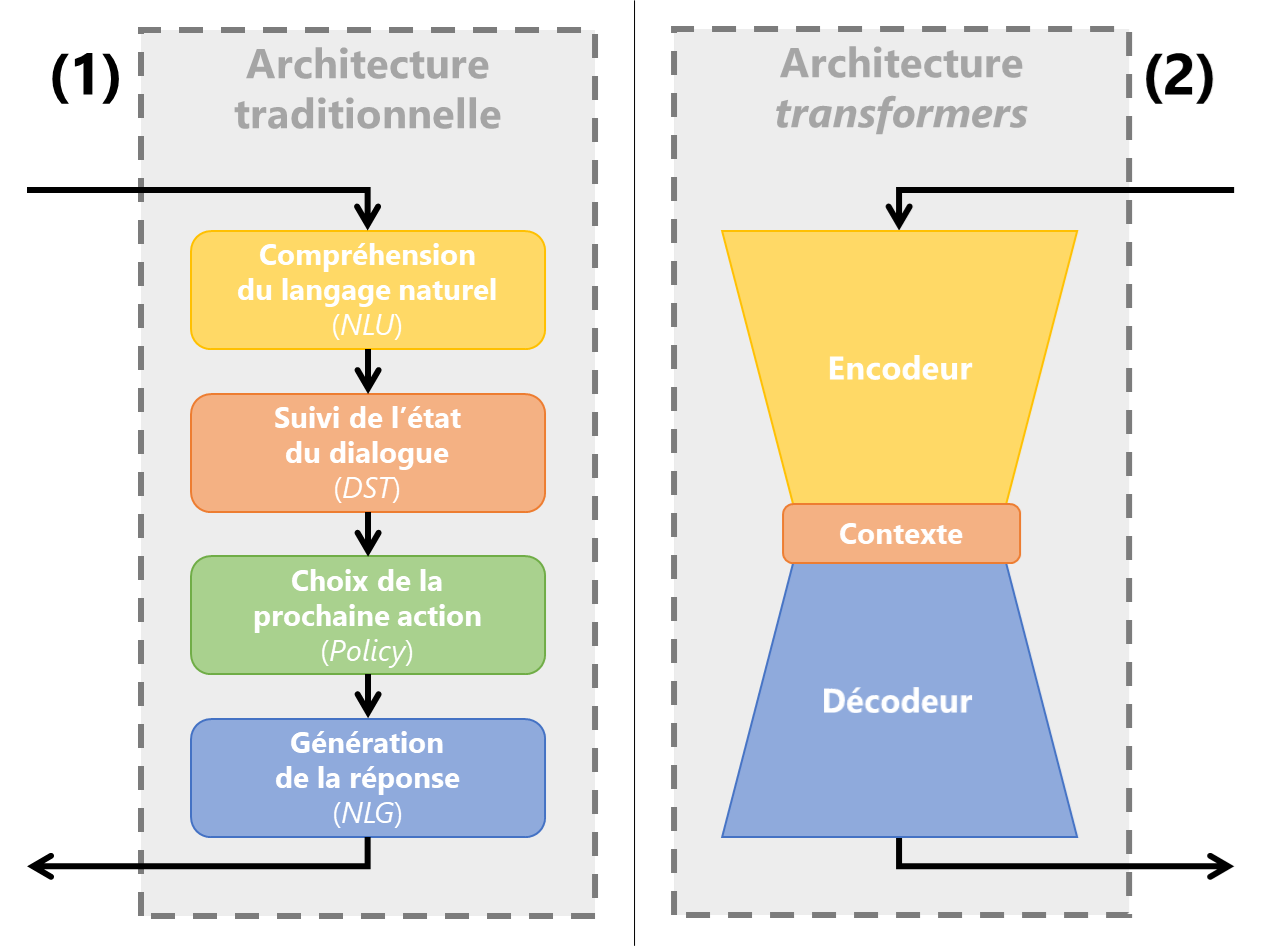
\includegraphics[width=0.90\textwidth]{figures/annexe-chatbots-architectures}
			\caption{
				Schéma illustrant les deux approches principales de conception d'un assistant conversationnel :
				\textbf{(1)} représente les \textbf{approches \textit{task-oriented}} à l'aide d'une architecture manipulant des états de dialogue ;
				\textbf{(2)} représente les \textbf{approches \textit{chat-oriented}} à l'aide d'une architecture à base de \textit{transformers}, encodant et décodant numériquement le dialogue et son contexte.
			}
			\label{figure:B.2-ANNEXE-CHATBOT-APPROCHES}
		\end{figure}
		
		
		%%%
		%%% Subsection B.2.1: Approches \textit{task-oriented}.
		%%%
		\newpage
		\subsection{Approches \textit{task-oriented}}
		\label{annex:B.2.1-ANNEXE-CHATBOTS-APPROCHES-TASK-ORIENTED}
		
			% Description.
			Les \textbf{approches orientées par tâches} (\textit{task-oriented}) considèrent la conversation comme une succession d'étapes menant à une action précise : le système est donc conçu pour collecter les informations nécessaires et interagir avec un moteur d'actions dans le but d'accomplir un objectif.
			Ces approches reposent généralement sur une modélisation explicite du parcours utilisateur, permettant ainsi de s'assurer de l'exécution pas à pas des actions intermédiaires de la tâche demandée.
			
			% Achitecture.
			La \textsc{Figure~\ref{figure:B.2-ANNEXE-CHATBOT-APPROCHES}} \textbf{(1)} représente l'architecture traditionnellement utilisée pour concevoir ce type d'assistants.
			Cette architecture est composée de éléments suivants :
			\begin{itemize}
				% NLU.
				\item le \textcolor{colorCarrotOrange}{\textbf{\texttt{NLU}}} (\textit{Natural Language Understanding}) :
					ce composant utilise un ensemble de concepts pour interpréter le dialogue de manière symbolique.
					Cette modélisation du dialogue, généralement implémentée à l'aide de méthodes supervisées, repose sur des détections de \textit{domaines} (\textit{thématique générale traitée}), des détections de \textit{sentiments} (\textit{positif, négatif ou neutre}), des détections d'\textit{intentions} (\textit{action exprimée par l'utilisateur, manifesté par le verbe d'action}), ou encore des extractions d'\textit{entités} (\textit{ensemble de mentions textuelles pertinentes}) (voir \cite{adamopoulou-moussiades:2020:overview-chatbot-technology}) ;
				% DST.
				\item le \textcolor{colorDarkPastelGreen}{\textbf{\texttt{DST}}} (\textit{Dialogue State Tracking}) :
					ce composant utilise les concepts détectés précédemment par le \texttt{NLU} (\textit{domaine}, \textit{sentiment}, \textit{intentions}, \textit{entités}) pour déterminer ou mettre à jour l'état de la conversation, et ainsi définir les actions possibles à partir de l'état en cours ;
				% PL.
				\item la \textcolor{colorDarkPastelGreen}{\textbf{\texttt{PL}}} (\textit{Policy Learning}) : 
					ce composant choisit la prochaine action de l'assistant parmi celle autorisée par le \texttt{DST} pour l'état en cours.
					Ce choix peut être réalisé à l'aide d'un ensemble de règles, d'un apprentissage supervisé ou encore d'un apprentissage par renforcement (voir \cite{brabra-etal:2022:dialogue-management-conversational}) ;
				% NLG.
				\item la \textcolor{colorSilverLakeBlue}{\textbf{\texttt{NLG}}} (\textit{Natural Language Generation}) :
					ce dernier composant affiche une réponse à l'utilisateur qui soit en adéquation avec l'action choisie par la \texttt{PL}.
					Cette réponse peut être paramétrée à l'avance ou être générée à la volée.
			\end{itemize}
			
			
			% Avantages et inconvénients.
			Cette approche est rudimentaire mais efficace, et elle est par conséquent fréquemment utilisée pour concevoir des assistants conversationnels dans un cadre industriel.
			\begin{itemize}
				\item[\faThumbsUp] Au sujet des avantages :
					% Implémentation facile.
					les différents composants de l'architecture sont simples à implémenter et à maintenir
					(\textit{ces différentes briques sont indépendantes et ont des fonctionnalités bien précises}) ;
					% Paramétrage facile.
					de nouvelles règles de dialogues peuvent facilement être ajoutées dans le système
					(\textit{du moins si les processus de ces tâches sont bien documentés}) ;
					% Mise sous contrôle.
					il est facile de contrôler le comportement de l'assistant
					(\textit{il suffit de restreindre les actions possibles dans le \texttt{DST}, de figer le choix de la \texttt{PL}, ou encore de déterminer à l'avance chaque réponse de la \texttt{NLG}}) ;
					% Infrastructure légère.
					cette architecture simple consomme peu de ressources en production (\textit{les modèles de détections et la gestion du dialogue peuvent tourner sur \texttt{CPU}}).
				\item[\faThumbsDown] Au sujet des inconvénients :
					% Couts initiaux.
					les coûts initiaux peuvent être importants (\textit{notamment en ce qui concerne la collecte et la modélisation des données d'apprentissage, ou encore la définition des parcours de dialogue pour des tâches non documentées}) ;
					% Modélisation sensible aux erreurs.
					la compréhension du langage est limitée (\textit{certaines erreurs ou ambiguïtés de langage rendent les détections du \texttt{NLU} non adaptées ou non performantes}) ;
					% Peu flexible.
					le dialogue est très peu flexible, et le périmètre de l'assistant est réduit à ce qui est modélisé (\textit{le dialogue peut être bloqué ou rejeté si aucune règle n'est prévue pour la demande de l'utilisateur ou pour l'état courant}).
			\end{itemize}
			
			\newpage
			
			% Exemple fictif.
			\begin{leftBarExamples}
				Pour illustrer nos propos, analysons la demande fictive suivante :
				\begin{quote}
					\begin{center}
						\textguillemets{\textit{
							Je veux réserver un billet de train pour Strasbourg.
						}}
					\end{center}
				\end{quote}
				\begin{itemize}
					\item le \texttt{NLU} pourrait détecter le domaine "\texttt{voyage}", l'intention "\texttt{réservation}" et les entités "$\textit{billet de train}_{\texttt{(produit)}}$" et "$\textit{Strasbourg}_{\texttt{(gare\_destination)}}$" ;
					\item le \texttt{DST} pourrait établir l'objectif de réserver un train, mais que les informations \texttt{(date\_départ)} et \texttt{(gare\_départ)} sont manquantes ;
					\item la \texttt{PL} pourrait décider de demander d'abord le complément d'information sur la gare de départ (\textit{et demandera la prochaine information plus tard}) ;
					\item la \texttt{NLG} pourrait sortir une phrase de réponse prédéfinie pour demander le complément d'information à l'utilisateur.
				\end{itemize}
			\end{leftBarExamples}
				
			% Exemples réels
			\begin{leftBarExamples}
				Nous pouvons citer les projets ou outils suivants :
				\begin{itemize}
					\item \texttt{RASA} (\cite{bocklisch-etal:2017:rasa-open-source}) et \texttt{WATSON} (\cite{hoyt-etal:2016:ibm-watson-analytics}) sont deux moteurs de dialogue basés sur une approche symbolique et manipulant des intentions et des entités ;
					\item \texttt{Assistant Virtuel SNCF} (\cite{sncf:2018:agent-virtuel-sncf}), \texttt{Google Assistant} (\cite{google:2016:google-assistant-your}) et \texttt{Alexa} (\cite{alexa-internet:2018:keyword-research-competitor}) sont des assistants connus pour être orientés par tâches, les deux derniers pouvant même être paramétrables par l'utilisateur final pour ses usages en domotiques ;
					\item \cite{yan-etal:2017:building-taskoriented-dialogue} décrivent un projet de conception d'un assistant conversationnel pour du commerce en ligne.
				\end{itemize}
			\end{leftBarExamples}
		
		
		%%%
		%%% Subsection B.2.2: Approches \textit{chat-oriented}.
		%%%
		\subsection{Approches \textit{chat-oriented}}
		\label{annex:B.2.2-ANNEXE-CHATBOTS-APPROCHES-CHAT-ORIENTED}
			
			% Description.
			Les \textbf{approches axées sur le dialogue} (\textit{chat-oriented} ou \textit{non-task-oriented}) sont utilisées pour favoriser des conversations ouvertes avec les utilisateur : le système n'est donc pas conçu pour répondre à un besoin spécifique, mais plutôt pour être en mesure de discuter avec un utilisateur sur des thématiques générales et de rebondir à chacun de ses messages de manière fluide .
			Afin de capturer la vaste diversité du langage, ces approches reposent majoritairement sur les capacités du \textit{Deep Learning}, notamment pour concevoir des modèles de langage permettant de capturer et de reproduire des séquences de phrases (voir \cite{ni-etal:2022:recent-advances-deep} et \cite{kumar-etal:2016:ask-me-anything}).
			
			% Achitecture.
			La \textsc{Figure~\ref{figure:B.2-ANNEXE-CHATBOT-APPROCHES}} \textbf{(2)} correspond à l'architecture \textit{transformers} (\cite{uszkoreit:2017:transformer-novel-neural}), communément utilisée pour représenter ce type d'assistants.
			Cette architecture est composée de deux réseaux de neurones :
			\begin{itemize}
				% Encodeur.
				\item un \textcolor{colorCarrotOrange}{\textbf{\texttt{encodeur}}} :
					ce premier réseau a pour objectif de traduire les séquences de mots du texte de l'utilisateur en une représentation numérique abstraite ;
				% Decodeur.
				\item le \textcolor{colorSilverLakeBlue}{\textbf{\texttt{décodeur}}} :
					ce second réseau a pour objectif de traiter la représentation numérique produite par l'encodeur dans le but de générer des séquences de mots pour former la réponse ;
				% Contexte.
				\item entre les deux, un \textcolor{colorDarkPastelGreen}{\textbf{\texttt{vecteur de contexte}}} :
					ce vecteur permet de maintenir la continuité de la co,versation entre deux échanges.
					L'encodeur se charge de mettre à jour le contexte tandis que le décodeur l'utilise pour adapter la génération de son texte.
			\end{itemize}
			
			
			% Avantages et inconvénients.
			Cette approche est plus difficile à mettre en place qu'une approche symbolique, mais elle dispose d'un plus grand potentiel.
			\begin{itemize}
				\item[\faThumbsUp] Au sujet des avantages :
					% Grande flexibilité.
					par conception, le système peut s'adapter à de nombreuses situations et offrir une expérience agréable à l'utilisateur
					(\textit{aucun blocage de l'état du dialogue, possibilité de personnaliser le dialogue, gestion plus simple de l'ambiguïté et des émotions, ...}) ;
					% Compréhension du langage.
					il n'a pas besoin d'interpréter le langage à l'aide d'une modélisation abstraite
					(\textit{cette interprétation est déduite de l'immense volume de textes utilisés à l’entraînement}) ;
					% Autres propriétés
					en utilisant des larges modèles de langage, des propriétés intéressantes peuvent apparaître
					(\textit{résumer ou traduire un texte, résoudre un calcul ou réaliser une déduction, large champ de connaissances, ...}).
				\item[\faThumbsDown] Au sujet des inconvénients :
					% Coûts techniques imports.
					les coûts d'entraînement et d'inférence du modèle sont conséquents
					(\textit{besoin d'une quantité démesurée pour l'apprentissage, besoin de \texttt{GPU} et d'une infrastructure technique musclée, ...}) ;
					% Mise sous contrôle
					la mise sous contrôle de l'assistant est difficile voire impossible
					(\textit{difficulté à évaluer les performances du modèle, possibilités d'hallucinations ou de générations offensantes, ...}).
			\end{itemize}
			
			% Exemples.
			\begin{leftBarExamples}
				Nous pouvons citer les projets ou outils suivants :
				\begin{itemize}
					\item \texttt{ChatGPT} (\cite{openai:2023:chatgpt}), \texttt{BARD} (\cite{google:2023:bard-chat-based}) et \texttt{LLAMA2} (\cite{touvron-etal:2023:llama-open-foundation}), trois solutions basées sur des larges modèles de langage permettant de discuter de presque tous les domaines ;
					\item \cite{kaddour-etal:2023:challenges-applications-large} détaillent une longue liste d'inconvénients et de défis pour l'utilisation de larges modèles de langage.
				\end{itemize}
			\end{leftBarExamples}
	
	
	%%%%%--------------------------------------------------------------------
	%%%%% Annexe B.3: Dilemme de conception et approches hybrides.
	%%%%%--------------------------------------------------------------------
	\section{Dilemme de conception et approches hybrides}
	\label{annex:B.3-ANNEXE-CHATBOTS-DILEMME}
		
		%%% Introduction: Description du dilemme.
		Dans la section précédente, nous avons pu voir que deux approches de conception se distingue :
		d'une part, il y a l'approche \textit{task-oriented}, basée sur une gestion symbolique du dialogue et permettant facilement de contrôler le comportement de l'assistant ;
		d'autre part, il y a l'approche \textit{chat-oriented}, basée sur un encodage/décodage numérique de la conversation et permettant une grande flexibilité dans les échanges avec l'utilisateur.
		Cependant, chaque approche possède les inconvénients de l'autre approche :
		en effet, l'approche \textit{task-oriented} est plutôt rigide, tandis que l'approche \textit{chat-oriented} est sensible aux dérives de comportement et aux risques d'hallucinations.
		Nous nous trouvons donc face à un dilemme de conception : \textbf{voulons-nous privilégier la fluidité du dialogue ou le contrôle du comportement ?}
		
		
		%%% Questionnement sur le niveaux d'automatisation.
		Ce choix cornélien questionne le \textbf{degré d'automatisation} que nous sommes prêts à accorder.
		En effet :
		\begin{itemize}
			\item si nous voulons plus de fluidité dans la conversation (\textit{pour améliorer l'ergonomie utilisateur, pour permettre de discuter de sujets plus généraux, ...}), nous nous tournerons davantage vers une approche \textit{chat-oriented}, et nous acceptons en échange de déléguer la gestion du dialogue ainsi que la génération de réponse à la machine ;
			\item à l'inverse, si nous avons besoin d'un contrôle plus fort (\textit{pour assurer la sécurisation des actions réaliser, pour garantir l'image de la marque, pour éviter les scandales, ...}), nous nous tournerons davantage vers une modélisation symbolique du dialogue, permettant de limiter les possibilités de divergence de la machine.
		\end{itemize}
		
		%%% Notes: complément sur le niveau d'automatisation.
		\begin{leftBarAuthorOpinion}
			% Dix niveaux d'automatisation.
			Pour estimer un \textbf{degré d'automatisation}, nous nous référons à \cite{sheridan-verplank:1978:human-computer-control} qui les classent en \textbf{dix niveaux} :
			\begin{enumerate}
				\item (\textit{faible}) La machine n'offre aucune assistance, l'opérateur doit tout faire seul ;
				\item La machine énumère exhaustivement les actions possibles, l'opérateur en choisit une et la réalise ;
				\item La machine suggère quelques actions possibles, l'opérateur en choisit une et la réalise ;
				\item La machine suggère une action à réaliser, l'opérateur peut la valider puis la réaliser ;
				\item La machine suggère l'action et la réalise si l'opérateur la valide ;
				\item La machine exécute automatiquement l'action au bout d'un certain temps si l'opérateur ne s'y oppose pas ;
				\item La machine exécute automatiquement l'action, puis informe l'opérateur ;
				\item La machine exécute automatiquement l'action, puis informe l'opérateur s'il l'a demandé ;
				\item La machine exécute automatiquement l'action, puis informe l'opérateur si la machine le juge pertinent ;
				\item (\textit{forte}) La machine exécute automatiquement l'action en ignorant l'opérateur.
			\end{enumerate}
			
			% Quatre fonctions à automatisées.
			De plus, \cite{parasuraman-etal:2000:model-types-levels} complètent l'estimation d'un degré d'automatisation en analysant \textbf{quatre aspects} :
			\begin{itemize}
				\item l'acquisition de l'information (\textit{est-ce que la machine collecte et sélectionne les informations pertinentes à porter à l'attention de l'opérateur ?}) ;
				\item l'analyse de l'information (\textit{est-ce que la machine examine les informations et propose les actions possibles à l'opérateur ?}) ;
				\item la prise de décision (\textit{est-ce que la machine choisit l'action à réaliser à la place de l'opérateur ?}) ;
				\item l'implémentation de l'action (\textit{est-ce que la machine réalise elle-même l'action ans aide de l'opérateur ?}).
			\end{itemize}
		\end{leftBarAuthorOpinion}
			
		% Retours aux chatbot.
		Ainsi, pour résoudre ce dilemme de conception d'un \textit{chatbot}, \textbf{diverses approches hybrides peuvent être mises en oeuvre}.
		
		\todo[inline]{A REDIGER: terminer les exemples...}
			
		% Exemples.
		\begin{leftBarExamples}
			TODO ...
			
			\begin{itemize}
				\item \textit{A REDIGER: approche à base de fouille de documents} (\cite{zhang-etal:2016:neural-information-retrieval})
				\item \textit{A REDIGER: utiliser l'encodeur pour le NLU} (\texttt{RASA v3.6+} (\cite{bocklisch-etal:2017:rasa-open-source}))
				\item \textit{A REDIGER: utiliser le décodeur pour la NLG} (\cite{gao-etal:2018:neural-approaches-conversational}, \cite{chen-etal:2017:survey-dialogue-systems})
				\item \textit{A REDIGER: entraîner la gestion de dialogue} (\cite{chen-etal:2017:survey-dialogue-systems}, \cite{brabra-etal:2022:dialogue-management-conversational})
			\end{itemize}
		\end{leftBarExamples}